\documentclass[11pt]{article}
% \usepackage{geometry}


\usepackage[margin=1.0in]{geometry}
\geometry{letterpaper}
\usepackage{graphicx}
\usepackage{amssymb}
\usepackage{float}
\usepackage{tabularx}
\usepackage{multicol}
\usepackage{hyperref}
\hypersetup{
    colorlinks,
    citecolor=black,
    filecolor=blue,
    linkcolor=black,
    urlcolor=black
}

\begin{document}

\begin{titlepage}
	\newcommand{\HRule}{\rule{\linewidth}{0.2mm}}
	\begin{center}
	\textsc{\LARGE McMaster University}\\[1.5cm]

	\textsc{\Large HydroSwarm}\\[0.5cm]
	\textsc{\large Software \& Mechatronics Capstone}\\[0.5cm]

	\HRule\\[0.4cm]
		{\huge\bfseries High Level System Design}\\[0.4cm]
	\HRule\\[0.4cm]

	\begin{minipage}[t][][t]{0.5\textwidth}
		\begin{flushleft} \large
			\emph{Authors:}\\
			Victor Velechovsky - \textit{001305263}\\
			Gabriel Potter - \textit{001429884}\\
			Amandeep Panesar - \textit{001431191} \\
			Taha Mian  - \textit{001417172}\\
			Nishanth Balamohan - \textit{001411319} \\
		\end{flushleft}
	\end{minipage}
	~
	\begin{minipage}[t][][t]{0.4\textwidth}
		\begin{flushright} \large
			\emph{Professor:} \\
			Dr. Alan Wassyng \\[0.4cm]
		\end{flushright}
	\end{minipage}\\[2cm]

	
\includegraphics[width=0.3\textwidth]{logo.png} \\
	{\large Last compiled on \today}
	\end{center}

\end{titlepage}

\tableofcontents
\listoffigures

\vfill
\begin{figure}[htbp]
   \centering
   \noindent\begin{tabularx}{\textwidth}{| >{\centering\arraybackslash}m{0.2\textwidth} | >{\centering\arraybackslash}m{0.2\textwidth} | >{\centering\arraybackslash}m{0.2\textwidth} | >{\centering\arraybackslash}m{0.285\textwidth} |}
   \hline 
   \textbf{Date} & \textbf{Revision} & \textbf{Comments} & \textbf{Author(s)} \\
   \hline
   Dec. 21 & 0.1 & Template added & Amandeep Panesar \\ \hline
   Dec. 21 & 0.2 & Added sections: Introduction, Team Members, Version Control, Workflow & All authors \\ \hline
   Dec. 21 & 0.3 & Added sections on component breakdown & All auhtors \\ \hline
   Dec. 23 & 1 & First revision & All authors \\ \hline
   \end{tabularx}
   \caption{Revision History}
\end{figure}

\newpage
\section{Introduction}
\subsection{Project Overview}
HydroSwarm is a swarm of autonomous robotic boats meant to carry out measurements over large bodies of water. For our project, these boats will be measuring water temperature, but the idea can be expanded to any number of other quantifiable measurements. Central to our work will be two major components. First, a small motorized boat, attached with a water temperature sensor, as well as a control unit that allows it to communicate with – and be controlled by – a centralized control unit. Second, a software package that can control a large group (\hyperref[sec:definitions]{swarm}) of these boats, with an algorithm focused on producing reliable, accurate, and fast measurements.\\

Our swarm will aim to cover large areas more quickly and cost-effectively than traditional products. To test the applicability of our project, we will demo it on a small scale body of water, such as a swimming pool, as well as develop a simulation to hypothetically prove the efficacy of the system on a larger scale.\\

Our project will be conducted between Fall 2018 –- Winter 2019 for our Engineering Capstone project at McMaster University, under the guidance of Dr. Alan Wassyng. We have four Software Engineering students, and one Mechatronics Engineering student. \\ \\

\subsection{Naming Conventions and Terminology}
\label{sec:definitions}
The following terms and definitions will be used throughout this document:
\begin{itemize}
% Alphabetical order is highly preferred as it eases user navigation
\item \textbf{System}: The entire software and hardware package - including the boats,
boat hardware, control software, and server running the control software
\item \textbf{Swarm}: A large group of objects (in our case, motorized boats) that can communicate and perform acts as a group
\item \textbf{Insect}: A member of the swarm (in our case, a single motorized boat)
\item \textbf{Simulation}: The simulation will be used for demo purposes, mainly to show that
the system is valid with a large number of insects.
\item \textbf{Researcher}: A user that is interested in the data that is returned from the survey.
\item \textbf{System Administrator}: A user that controls the parameters of the \hyperref[sec:definitions]{\textbf{swarm}}.
\item \textbf{G.P.S.}: Global Positioning System
\item \textbf{Coverage area}: The area in which the insects are confined. This defines that space that the user wants to track and measure.
\item \textbf{API}: Application Programming Interface
\end{itemize}

\subsection{Project Scope}
Due to time and financial constraints, defining the project's scope is essential to ensure the project is feasible. One way we are scoping the project is the type of data we collect with each insect. We are only collecting temperature and location data. Another way we are scoping the project is restricting the area of the survey. Insects can travel only a maximum distance (approximately covering the size of a swimming pool) from the starting point. The type of water that the swarm will be deployed on is fresh water. We are using existing RC boats, and will not be building our own. We will also rely on other third-party components, such as embedded microcontrollers and transceivers. \\

See the Requirements Document for a more detailed explanation of the project scope.
%TODO REFERENCE REQ DOC HERE

\section{System Description}

\subsection{System Architecture}
The system will be comprised of a server that controlled a group of client insects.
The insects will be responsible for taking measurements, tracking their position,
and moving as directed by the server.
The server will be responsible for determining how insects should move, and when to take
measurements. It will also contain a User Interface, to configure system parameters and
display results to the user, as well as a simulation of how the system would run under
various test conditions (arbitrary coverage areas and arbitrary insect counts).

With this decomposition, the insects will largely be "dummy" components - most of the
business logic will be performed by the server. It also ensures that each component
can be designed relatively independently (as long as it adheres to the correct communication
API).


\subsection{System Variables}
Refer to Requirements document Figure 3.
\subsection{Subsystems}
The system will be broken down into the following subsystems. 
\begin{itemize}
\item \textbf{Simulation}
\item \textbf{Insect Tracking/Positioning}
\item \textbf{Insect Motor Control}
\item \textbf{Insect Measurement Sensors}
\item \textbf{Server Communication Interface}
\item \textbf{Insect Communication Interface}
\item \textbf{User Interface}
\item \textbf{Area Coverage Algorithm}
\item \textbf{Data Storage}

\end{itemize}

\begin{figure}[H]
   \centering
   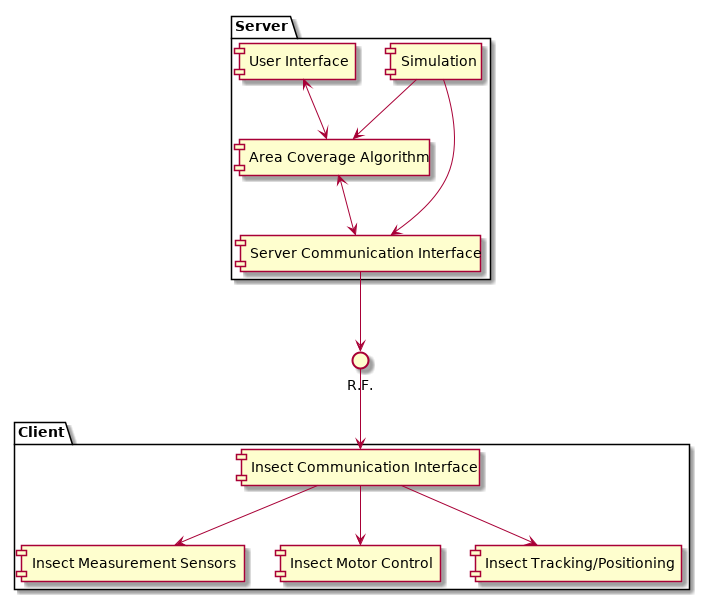
\includegraphics[width=0.8\textwidth]{diagram/component-diagram.png}
   \caption{Subsystem Breakdown}
   \label{fig:sub}
\end{figure}
\subsection{Use Cases}
The diagram including all use cases can be found in Figure \ref{fig:usecase}. The user-instantiated ones will be described in detail below.
\begin{figure}[H]
   \centering
   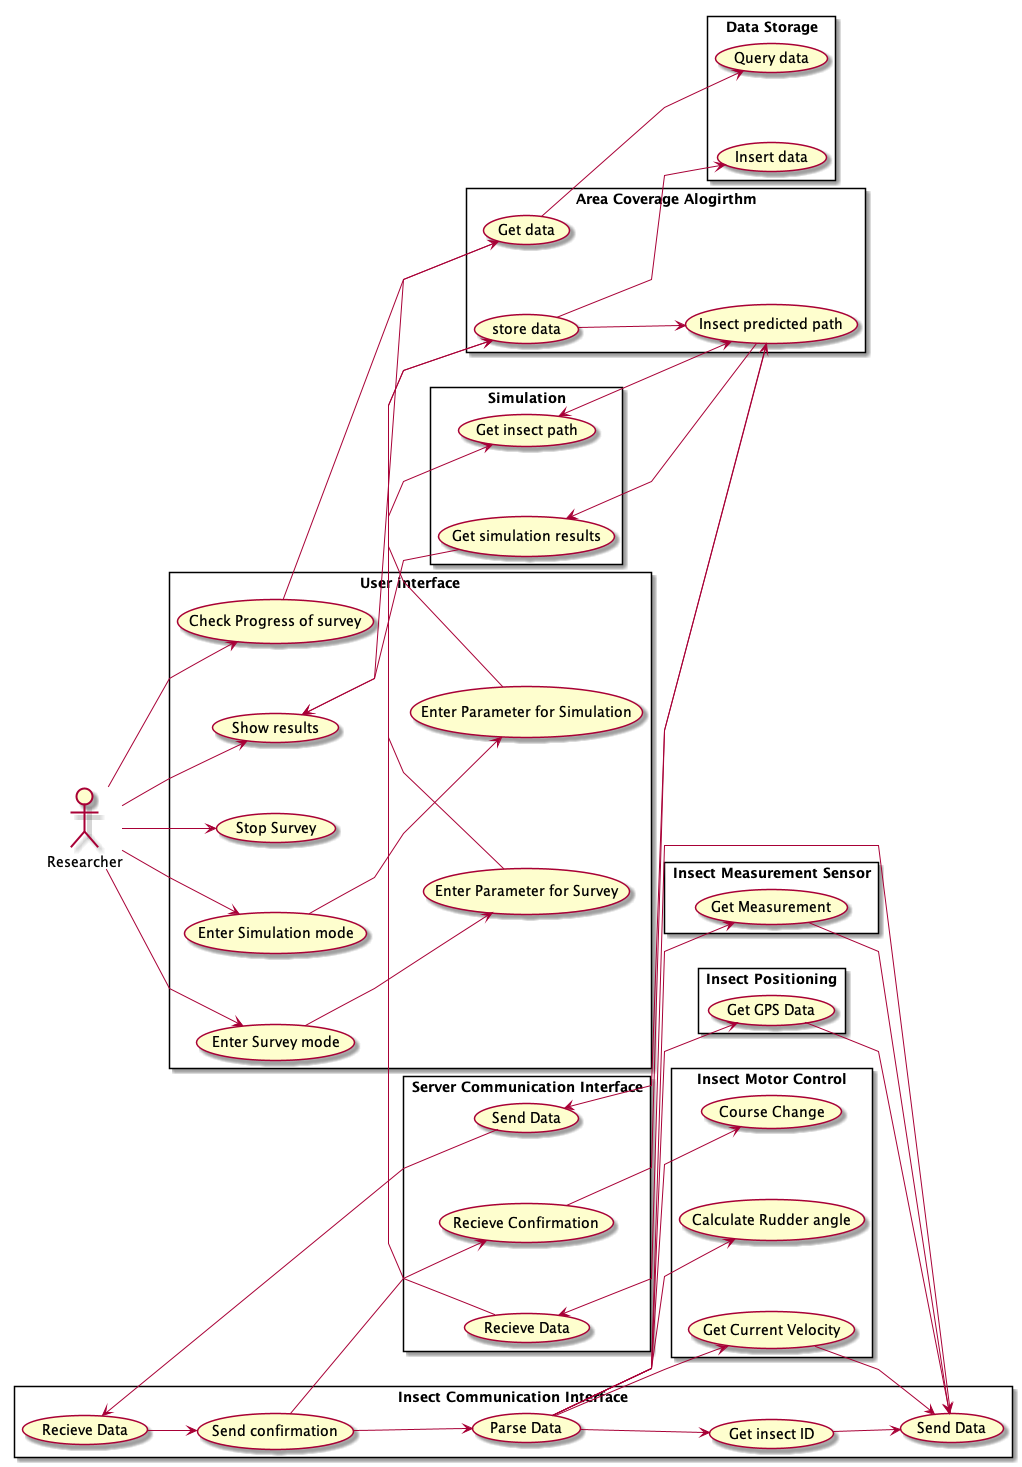
\includegraphics[width=\textwidth, height=16.5cm]{diagram/usecase.png} % requires the graphicx package
   \caption{Use Case Diagram}
   \label{fig:usecase}
\end{figure}

\subsubsection{Conduct a Survey} 
Researcher can request to start a survey with custom defined parameters and begin to conduct a survey. The user interface will then show the results after the insects have fully surveyed the area.
\begin{figure}[H]
   \centering
   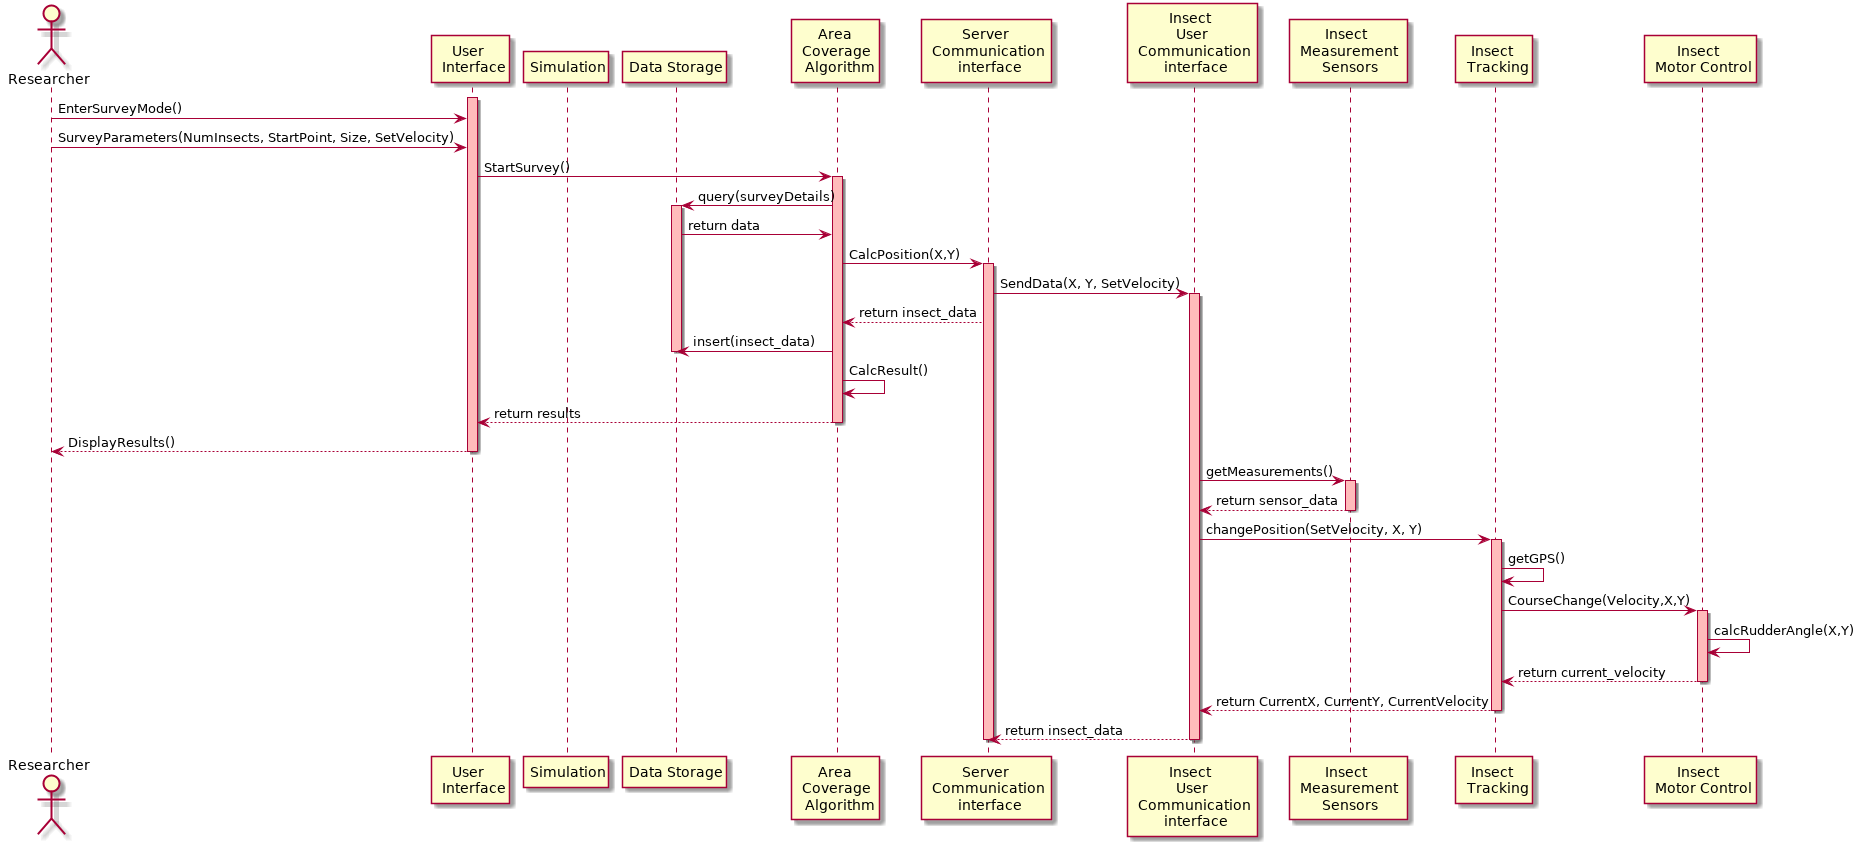
\includegraphics[width=18cm, height=12cm]{diagram/survey.png}
   \caption{Sequence Diagram for conducting a survey}
   \label{fig:stop}
\end{figure}
\subsubsection{Stop a Survey}
Researcher can request to stop a survey while it started. While in Survey mode in the user interface, the researcher can request the survey to be stopped, and then the survey is terminated.
\begin{figure}[H]
   \centering
   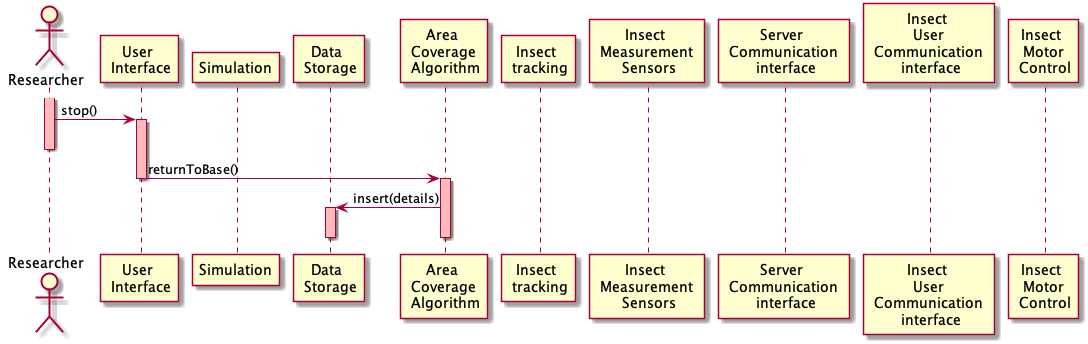
\includegraphics[width=\textwidth]{diagram/stopsequence.png}
   \caption{Sequence Diagram for Stopping a survey}
   \label{fig:stop}
\end{figure}

\subsubsection{Inspect Survey Output}
Researcher can view the data that was retrieved during the survey. The user interface displays all the data collected from the survey, as well as graphical representations of how the insects collected data.
\begin{figure}[H]
   \centering
   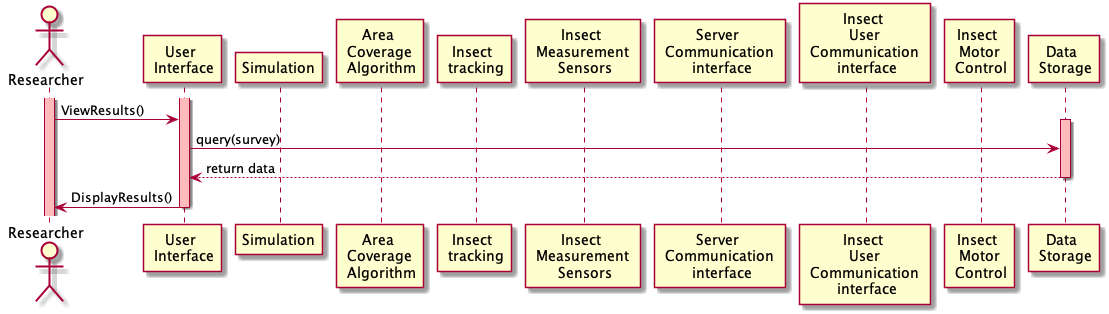
\includegraphics[width=\textwidth]{diagram/outputsequence.png}
   \caption{Sequence Diagram for Checking survey Results}
   \label{fig:stop}
\end{figure}


\subsubsection{Check Progress of Survey}
Researcher can also check the progress of surveys as they are being conducted. The user interface displays real time data of the location of insects, as well as the amount of survey that is completed.
\begin{figure}[H]
   \centering
   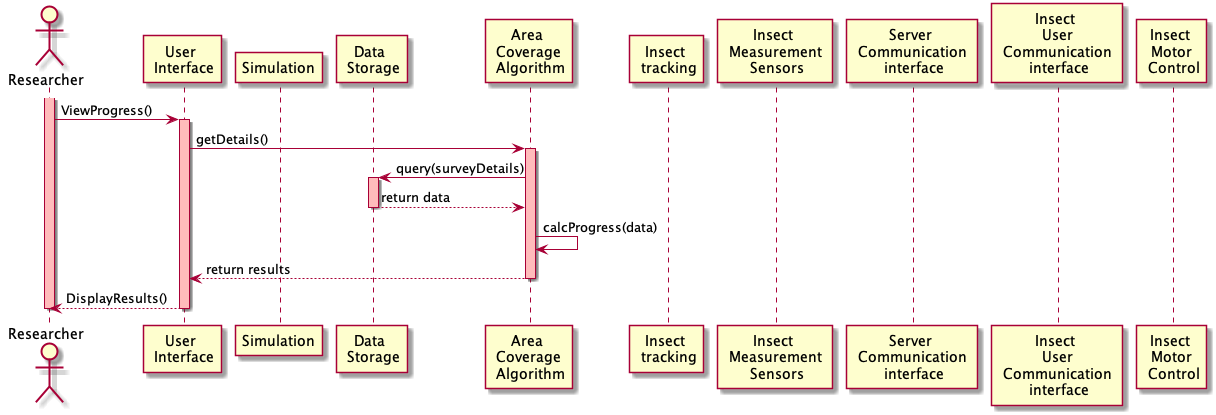
\includegraphics[width=\textwidth]{diagram/checksequence.png}
   \caption{Sequence Diagram for Checking survey progress}
   \label{fig:stop}
\end{figure}


\subsubsection{Run a Simulation}
Researcher may want to run a simulation to visualize the behaviour of the swarm in a defined body of water. The user interface allows for a simulation mode, where users can input parameters and run a simulation before actually deploying the swarm, and conducting the survey.
\begin{figure}[H]
   \centering
   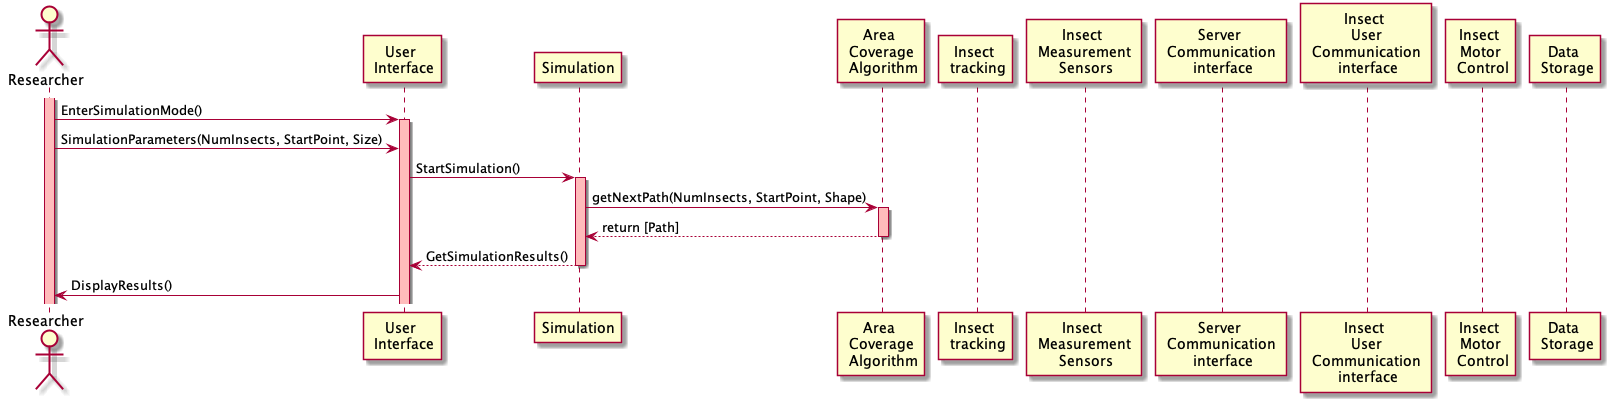
\includegraphics[width=\textwidth]{diagram/sequence.png}
   \caption{Sequence Diagram for Running a simulation}
   \label{fig:stop}
\end{figure}


\subsection{Behaviour Description}
As the behaviour of the system has been discussed previously, this section will describe the expected user behaviour and how they will interact with the system.

This section breaks down operation of the system into examples of typical and expected use cases, under \textit{Normal Operation}, and
unexpected or edge cases, under \textit{Abnormal Operation}. It explores how a properly designed system should respond to abnormal operations
in order to ensure reliability and robustness.

\subsubsection{Normal Operation}
When the server application is first executed, there will be various options available to the user to set up operation of the system. As described
throughout this document and the requirements document, there will be options for defining a coverage area and a starting point. There will also
be a mechanism for connecting insects with the system so that they are prepared to be controlled by the server.

Once all settings have been appropriate picked, the user will start the coverage module, which will begin moving the drones and collecting
measurements. Once the coverage area is fully covered, the system will notify the user of its successful completion, and a visual display of the
temperature measurements will be displayed.

The user will be able to observe the measured data, as well as export it for external use. Once satisfied, the user will exit the application.
\subsubsection{Abnormal Operation}
Abnormal operations will occur if there are software bugs, mechanical failures, or failures of the user to properly define configuration parameters (involving the coverage area and starting point). For example, the user may input a coverage area that is larger than the physical area being measured. 
This could result in the boats hitting a physical boundary, or leaving the physical coverage area, which could be a safety concern.

Another pertinent example would be a boat that encounters a mechanical failure, relating to its motors, measuring devices, or micro-controller.
\subsubsection{Error Handling}
Due to financial and time constraints, we will not be able to detect an invalid coverage area or starting point. As such, we may not always be able
to detect if a boat has entered or is trying to enter an inappropriate area. We will, however, be able to detect mechanical failures in the boats.
These can be communicated to the server (a lack of timely response from an insect would also imply some failure with the boat). When a failure occurs,
the server will attempt to shut down all motor and measurement functionality of that insect. Depending on the nature of the issue, the system
may attempt to continue operation with all other insects, or such down the system entirely, if deemed necessary.

If an insect experiences a failure with its measuring device, but appears healthy otherwise, the system will attempt to continue operation with
all other insects. In more serious hardware failures, the system will cease all operations, and display a message to the user, via the User Interface,
notifying them of the error.
\section{Subsystems Overview}

This section covers a brief overview of the purpose and overall functionality of each subsystem, as well as the expected
monitored and controlled variables.

\subsection{Area Coverage Algorithm}
\subsubsection{Description}
The area coverage algorithm is responsible for deciding how to move the insects, in order to map the coverage area as quickly and
efficiently as possible. At the beginning of operation, it will be provided with all the relevant context (regarding the coverage area,
insects, etc), and then it will begin computing directions for each individual insect to move in. The algorithm may use the current
state of the system (insect locations, measurements made, etc) to make more informed decisions as time progresses.\\

\begin{figure}[H]
   \centering
   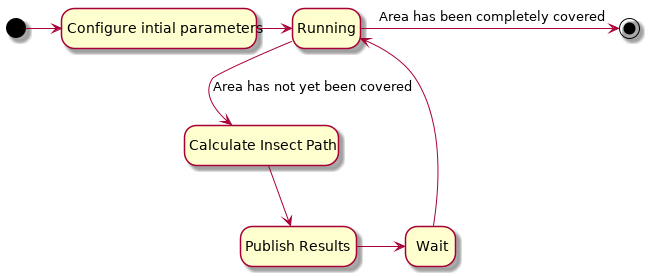
\includegraphics[width=0.7\textwidth]{diagram/areacov.png}
   \caption{State machine diagram of the component functionality}
   \label{fig:algorithm-fsm}
\end{figure}

\subsubsection{Controlled Variables}

\textbf{Movement directions}: At a regular interval, the algorithm decides on a position (represented as
x, y coordinates) for each individual insect to move to, in order to ensure that area coverage is efficient and accurate \\

\subsubsection{Monitored Variables}

\textbf{Coverage area}: A two dimensional shape that defines the coverage area of the system \\
\textbf{Starting point}: This defines a point within the coverage area, around which the insects are placed initially\\
\textbf{Number of healthy insects}: The number of functioning insects that are connected to the system\\
\textbf{Measurements made}: A history of measurements made by the insects. Each measured quantity will contain information about the
temperature value, the insect that made the measurement, the time it was made, and the location it was made at. Initially, this will
be empty\\
\textbf{Locations visited}: A history of all locations that insects have successfully moved to and made measurements at\\

\subsection{Insect Motor Control}
\subsection{Input}
\textbf{Coordinates}: Desired position.
\subsection{Output}
\textbf{Velocity}: Actual velocity measured by the on board accelerometer.
\subsection{Description}
The motor control subsystem will provide a means for controlling the velocity of each insect. Each boat in the swarm will have this subsystem which will be responsible for interpreting the desired speed and direction data received from the communications and positioning subsystems and enacting those instructions by sending the appropriate signals to the motors present on each boat. Important hardware contained in this subsystem includes:
\begin{itemize}
\item \textbf{Micro-controller} - originating point for motor control signals and interface to the communications subsystem
\item \textbf{H-bridge circuitry} - facilitates simple motor direction control and protects micro-controller from excessive current
\item \textbf{Motors} - control the direction and speed of the boat
\end{itemize}
\begin{figure}[H]
   \centering
   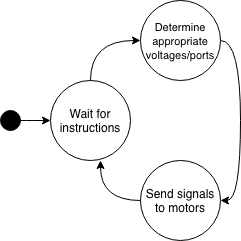
\includegraphics[width=0.4\textwidth]{img/motor_ctrl_fsm.png}
   \caption{Motor Control FSM}
   \label{fig:fsm}
\end{figure}
The motor control interface in software should hide all internal motor control details such as voltages, ports, number of motors, etc. This is information that has no relevance to other subsystems and therefore will be wholly contained within the motor control subsystem itself. The interface should only contain data on the boats desired speed and direction. This will ensure seamless adoption of different motor configurations should the need arise, without having make changes to other subsystems other than the motor control subsystem itself.

\subsubsection{Monitored Variables}
\textbf{Desired velocity}: Subsystem uses this variable in its calculations.

\subsubsection{Controlled Variables}
\textbf{Motor signals}: This subsystem has control over the hardware ports driving the motor control signals.


\subsection{Server Communication Interface}
\subsubsection{Input}
\textbf{Coordinates:} The coordinates for the next position, and set velocity. 
\subsubsection{Output}
\textbf{Insect Data:} A data object returned from the Insect Communication Subsystems such as temperature, velocity, and position.
\subsubsection{Description}
The server communication subsystem is responsible for communicating important information from the server to the insect. In addition, data will also be received from the insect which might contain information such as position, temperature, and velocity.  The data transmitted to the insect will also follow a similar structure and include data such as desired speed and position. The hardware components involved in the interaction will include a micro-controller and RF transceiver which has the ability to send and receive data. 

\begin{figure}[H]
   \centering
   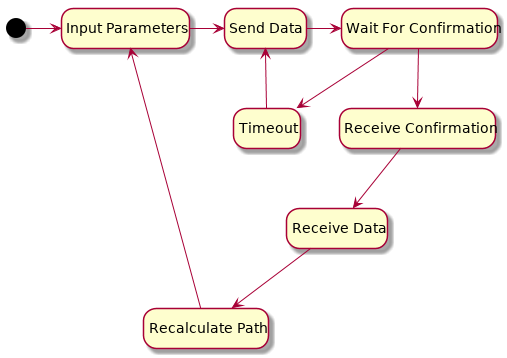
\includegraphics[width=0.5\textwidth]{img/serverCom.png}
   \caption{Server Communication FSM}
   \label{fig:fsm}
\end{figure}

\subsubsection{Controlled Variables}
\textbf{Movement Directions}: At a regular interval, the algorithm decides on a position (represented as
x, y coordinates) for each individual insect to move to, in order to ensure that area coverage is efficient and accurate \\
\textbf{Movement Velocity}: The user defined velocity is used to set the speed of the insects.

\subsubsection{Monitored Variables}
\textbf{Insect ID}: A unique identifier that distinguishes the insects from each other. \\  
\textbf{Sensor Output}: Data logged by the sensors on board the insect (i.e temperature sensor). \\
\textbf{Insect Velocity}: The actual velocity reported by the on board accelerometer. \\ 
\textbf{Current Position}: The actual position reported by the insect tracking/position sub system. \\

\subsection{Insect Communication Interface}
\subsubsection{Input}
\textbf{Insect Data:} An insect data object that contains temperature logged,current position, id, and velocity. 
\subsubsection{Output}
\textbf{Coordinates:} Data sent from the server which contains the position.
\textbf{Velocity:} Data sent from the server which contains desired velocity.
\subsubsection{Description}
The insect communication subsystem is responsible for communicating vital information from the insect to the server. The data  transmitted will include sensor data, GPS coordinates,and accelerometer output. The data received from the server will include information such as speed and direction based on algorithm output. The hardware components interacting with this subsystem will include a micro-controller and RF transceiver which will have the ability to send and receive data The input will include data that will be sent to the server such as temperature logged,current position, id, and velocity. The output will be the data received by the server such as desired velocity and position. 

\begin{figure}[H]
   \centering
   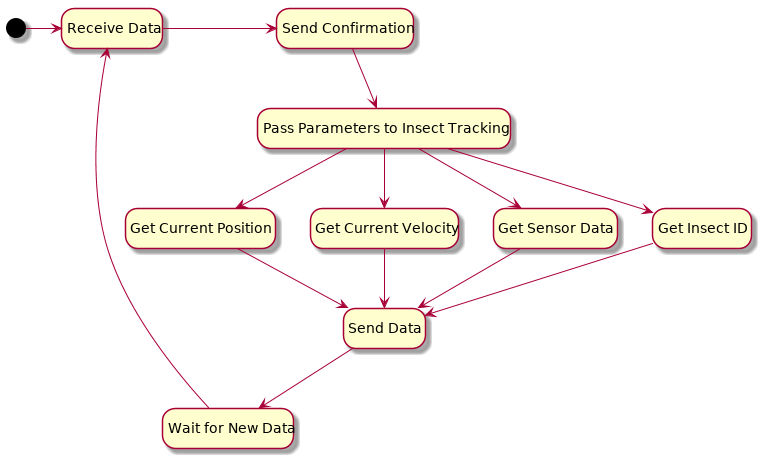
\includegraphics[width=0.75\textwidth]{diagram/insectCom.png}
   \caption{Insect Communication FSM}
   \label{fig:fsm}
\end{figure}

\subsubsection{Controlled Variables}
\textbf{Insect ID}: A unique identifier that helps the server distinguish between insects. \\  
\textbf{Sensor Output}: Data logged by the insect measurement sensors sub system. \\
\textbf{Insect Velocity}: The actual velocity reported by the motor control sub system. \\ 
\textbf{Current Position}: The actual position reported by the insect tracking/position sub system. \\


\subsubsection{Monitored Variables}
\textbf{Movement Directions}: X, and Y coordinates sent from the server which are constantly being updated. \\
\textbf{Movement Velocity}: The velocity set by the user which is monitored and compared to the insect velocity. \\



\subsection{Insect Tracking/Positioning}
\subsubsection{Description}
The insect tracking and positioning subsystem is responsible for determining the position of each individual insect within the area of coverage, and ensuring that the boat is adhering to the desired velocity specified by the area coverage algorithm. Therefore each insect/boat will be equipped with this subsystem. Hardware components of this subsystem include the micro-controller and GPS module. This subsystem will interact with the communications subsystem and the motor control subsystem. It will send GPS coordinates and velocity to the communications subsystem, and it will calculate slight adjustments to the boat velocity and send these updates to the motor control subsystem.
\begin{figure}[H]
   \centering
   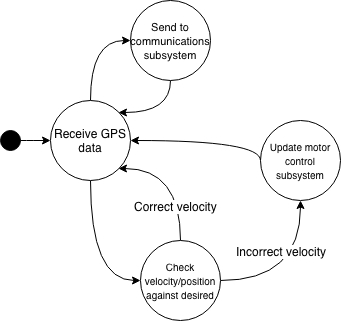
\includegraphics[width=0.5\textwidth]{img/position_ctrl_fsm.png}
   \caption{Tracking/Positioning FSM}
   \label{fig:fsm}
\end{figure}

\subsubsection{Controlled Variables}
\textbf{Insect position and velocity}: This subsystem is solely responsible for measuring and updating the current values of position and velocity.\\
\textbf{Adjusted velocity}: Subsystem uses this variable to make slight velocity adjustments and path corrections.

\subsubsection{Monitored Variables}
\textbf{Desired velocity}: Subsystem monitors this to ensure the boat is hitting target.

\subsection{Insect Measurement Unit}
The insect measurement unit will consist of the temperature sensor. The thermistor within the sensor will collect data according to the change in resistance which is then read by the sensor as a temperature reading. The sensor will periodically transmit the temperature data via interaction with the communications subsystem.

\subsubsection{Monitored Variable}
\textbf{Measured Temperature}: This is the data that is collected and transmitted by the temperature sensor. 

\subsection{User Interface}
\subsubsection{Inputs}
Same as Controlled Variables
\subsubsection{Outputs}
\textbf{Graph}: Graphical representation of collected data.
\subsubsection{Description}
The User Interface subsystem is how users will interact with the Area Coverage Algorithm. Once launched the user will have the options to either run a simulation of the swarm or to view the data collected by the insects. If the simulation mode is selected, the user will select the body of water then select the number of insects in the drone. From there the UI will display the Simulation from the data sent to the Area Coverage Algorithm. If operational mode is selected, the UI will display the temperature readings and locations of the insects in the body of water in real-time via the communications subsystem. This will allow the user to get a real-time view of the change in temperature throughout the body of water.
\subsubsection{Monitored Variables}
\textbf{Progress of Survey}: The graphical representation of the current progress of the survey.\\
\textbf{Results of Simulation}: The graphical results of the simulation.\\
\textbf{Results of Survey}: The graphical results of the survey.
\subsubsection{Controlled Variables}
\textbf{Number of Insects}: Number of insects in the survey \\
\textbf{Size of Survey}: Size of area that the survey will be conducted in.\\
\textbf{Mode Selection}: Researcher enters which mode they would like to enter. \\
\textbf{Starting Point}: Researcher enters relative starting point of survey.

\begin{figure}[H]
   \centering
   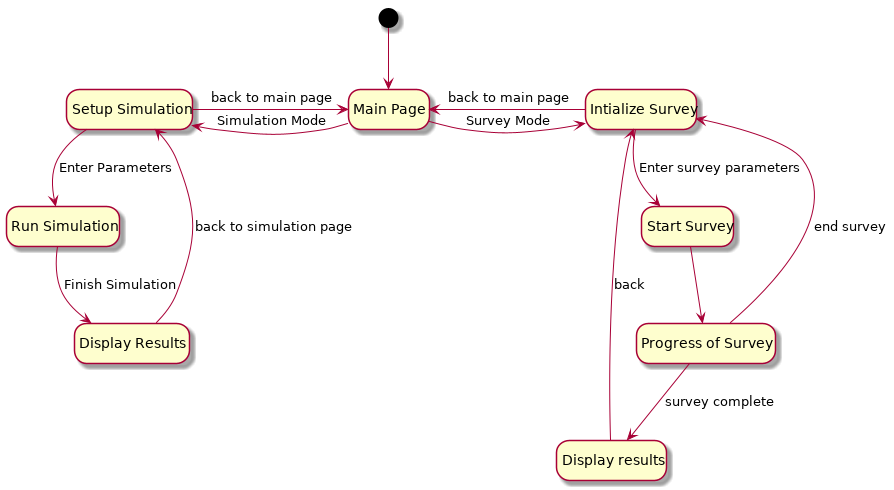
\includegraphics[width=0.9\textwidth]{diagram/userint.png}
   \caption{State machine for the User interface subsystem}
   \label{fig:algorithm-fsm}
\end{figure}

\subsection{Data Storage}
\subsubsection{Inputs}
\textbf{Inserted Data:} Data that needs to be stored. 
\subsubsection{Outputs}
\textbf{Queried Data:} Data that is queried and needs to be displayed to the user interface
\subsubsection{Description}
The Data storage subsystem will store data for every survey, it will store the temperature data along with the X, and Y coordinates from where the data was collected. Data storage will also store details of each survey.
\subsubsection{Controlled variables}
\textbf{Insect data Object:} Data object that includes details of a specific survey. \\
\textbf{Survey data Object:} Data object includes details of survey session.

\subsection{Simulation Subsystem}
\subsubsection{Input} Same as controlled variables
\subsubsection{Output} Same as monitored variables
\subsubsection{Description}
The Simulation subsystem will allow users to visually see the behaviour of insects during a survey. Users will have to define dimensions of the body of water being surveyed, also a starting point must be chosen. Users must also the enter the amount of insects that the simulation will use. The simulation will use the Area Coverage Algorithm subsystem to determine the next location of all insects, and will give an approximate time of competition. The history of an insect's path will also be stored, all this information will be displayed to the user in the user interface subsystem. In this case the inputs of the simulation subsystem will be controlled variables, and the output will be the monitored variables.
\subsubsection{Controlled Variables}
\textbf{Dimensions of survey:} The size of the boundaries of the simulation, this will be defined as a rectangle where user defines length and width. \\
\textbf{Starting position:} The starting position of all insects (starting point of the survey),. User will define a coordinates within the defined survey area. \\
\textbf{Number of insects:} The amount of insects that will be used in the survey.

\subsubsection{Monitored Variables}
\textbf{The location Insects:} At every time instance the current location of the insect. \\
\textbf{Path of insects:} The path that each insect used during the simulation.\\
\textbf{Estimated Time of completion:} The 
approximate time it takes to complete the survey.

\begin{figure}[H]
   \centering
   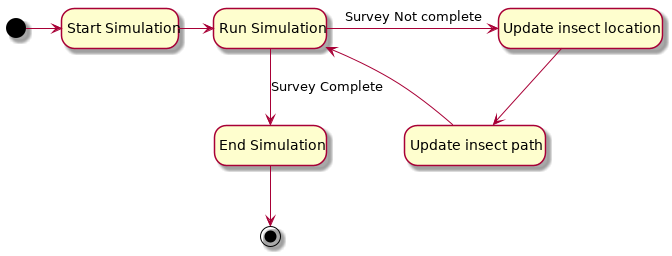
\includegraphics[width=0.7\textwidth]{diagram/simulation.png}
   \caption{State machine for the simulation subsystem}
   \label{fig:algorithm-fsm}
\end{figure}




\section{Constants}

Our final demonstration will involve a number of set constraints, which are outline in this section. They are mentioned because some 
of them will be represented in the software code.

It is likely that many more constraints will be discovered, particularly with the hardware components, that will be uncovered later in the
development process. These will be presented in the component design document, and later, in Revision 1 of this document. For now, we list only
constraints that we are reasonably certain about with the knowledge we currently have.

\begin{itemize}
    \item \textbf{Coverage area}: The coverage area for our demo
    will be the \textbf{McMaster swimming pool - a $50m$ x $22.5m$} facility located in the \textit{Ivory Wynne Center}. This will be
    represented in the code that handles coverage areas - it will be limited to a rectangle of this size.
    
    \item \textbf{Number of insects}: Due to financial and time constraints, our demonstration will have \textbf{three} physical insects.
    
    \item \textbf{Demonstration time}: The demonstration will be limited to \textbf{ten minutes} (or less, if the demo successfully finished before
    that time).
    
    \item \textbf{Distance between adjacent locations in the coverage area}: The coverage area will be considered in discrete \textbf{$1m$ x $1m$} increments. Insect will move between positions in increments of $1m$ at a time.
    
    \item \textbf{Movement direction}: If the coverage area is considered as a 2-dimensional matrix of positions, the insects will move up, down, left
    or right, \textit{but not diagonally}.
\end{itemize}

\section{Class Responsibility Collaboration (CRC) Cards}
The following sections will include one CRC card for each subsystem. A CRC card contains information pertaining to which requirements a subsystem is responsible for and which subsystems one would collaborate with. This will be used for testing purposes and to track where a given requirement is satisfied. A requirement does not have to be satisfied completely by one subsystem, but a majority of the work must be done by that subsystem.

\subsection{Area Coverage Algorithm}
\begin{table}[H]
\centering
\label{my-label}
\begin{tabular}{ | >{\raggedright\arraybackslash}p{0.4\textwidth} | >{\raggedright\arraybackslash}p{0.4\textwidth} | }
\hline
\multicolumn{2}{|c|}{\textbf{Hydroswarm}}             \\ \hline
\textbf{Responsibilities:} & \textbf{Collaborators:} \\ \hline
\begin{itemize}
\item \textbf{Functional 5}: Each insect in the system shall be maneuverable such that it
can move to any position (x, y) on the surface of the water
\item \textbf{Functional 6}: The system shall be able to plan and control the paths of insects
such that redundant measurements are not made and there are no collisions
\item \textbf{Non-Functional 3}: The system must collect data within a reasonable maximum amount of
time
\item \textbf{Non-Functional 4}:  The system must collect data for a long enough amount of time
without failing
\end{itemize}
&
\begin{itemize}
\item Server Communications
\item Data Storage
\item User Interface
\end{itemize} \\ \hline
\end{tabular}
\caption{Area Coverage Algorithm CRC Card}
\end{table}

\subsection{Insect Motor Control}

\begin{table}[H]
\centering
\label{my-label}
\begin{tabular}{ | >{\raggedright\arraybackslash}p{0.4\textwidth} | >{\raggedright\arraybackslash}p{0.4\textwidth} | }
\hline
\multicolumn{2}{|c|}{\textbf{Hydroswarm}}             \\ \hline
\textbf{Responsibilities:} & \textbf{Collaborators:} \\ \hline
\begin{itemize}
\item \textbf{Functional 5}: Each insect in the system shall be maneuverable such that it
can move to any position (x, y) on the surface of the water
\item \textbf{Functional 6}: The system shall be able to plan and control the paths of insects
such that redundant measurements are not made and there are no collisions
\item \textbf{Non-Functional 12}: The insects will not travel too quickly
\end{itemize}
&
\begin{itemize}
\item Insect Communications
\item Insect Tracking/Positioning
\item Area Coverage Algorithm
\end{itemize} \\ \hline
\end{tabular}
\caption{Insect Motor Control CRC Card}
\end{table}
\subsection{Server Communication}
\begin{table}[H]
\centering
\label{my-label}
\begin{tabular}{ | >{\raggedright\arraybackslash}p{0.4\textwidth} | >{\raggedright\arraybackslash}p{0.4\textwidth} | }
\hline
\multicolumn{2}{|c|}{\textbf{HydroSwarm}}             \\ \hline
\textbf{Responsibilities:} & \textbf{Collaborators:} \\ \hline
\begin{itemize}
\item \textbf{Functional 9:} If an insect loses a critical function for autonomous operation it shall have the ability to be manually overridden and controlled by
the user.
\item \textbf{Functional 10:}  If an insect loses critical functionality such as communication,
sensing, or movement, the remaining operational insects should operate as if that
insect is no longer part of the swarm.
\item \textbf{Non Functional 5:} The swarm must be able to work with an arbitrary number of
insects.
\item \textbf{Non Functional 7:} The user shall be able to pair insects to the server.
\item \textbf{Performance 3:} Response time between the server and insects should not exceed over one second
\end{itemize}
&

\begin{itemize}
\item Area Coverage Algorithm
\item User Interface
\item Insect Communication
\end{itemize} \\ \hline
\end{tabular}
\caption{Server Communication Card}
\end{table}
\subsection{Insect Communication}
\begin{table}[H]
\centering
\label{my-label}
\begin{tabular}{ | >{\raggedright\arraybackslash}p{0.4\textwidth} | >{\raggedright\arraybackslash}p{0.4\textwidth} | }
\hline
\multicolumn{2}{|c|}{\textbf{HydroSwarm}}             \\ \hline
\textbf{Responsibilities:} & \textbf{Collaborators:} \\ \hline
\begin{itemize}
\item \textbf{Functional 9:} If an insect loses a critical function for autonomous operation it shall have the ability to be manually overridden and controlled by
the user.
\item \textbf{Functional 10:}  If an insect loses critical functionality such as communication,
sensing, or movement, the remaining operational insects should operate as if that
insect is no longer part of the swarm.
\item \textbf{Functional 2:} Each insect in the swarm must be able to provide its current location
\item \textbf{Non Functional 5:} The swarm must be able to work with an arbitrary number of
insects.
\item \textbf{Non Functional 7:} The user shall be able to pair insects to the server.
\item \textbf{Performance 3:} Response time between the server and insects should not exceed over one second
\end{itemize}
&

\begin{itemize}
\item Server Communication
\item Insect Motor Control
\item Insect Tracking/Positioning
\item Insect Measurement Sensors
\end{itemize} \\ \hline
\end{tabular}
\caption{Insect Communication CRC Card}
\end{table}

\subsection{Insect Tracking/Positioning}

\begin{table}[H]
\centering
\label{my-label}
\begin{tabular}{ | >{\raggedright\arraybackslash}p{0.4\textwidth} | >{\raggedright\arraybackslash}p{0.4\textwidth} | }
\hline
\multicolumn{2}{|c|}{\textbf{Hydroswarm}}             \\ \hline
\textbf{Responsibilities:} & \textbf{Collaborators:} \\ \hline
\begin{itemize}
\item \textbf{Functional 2}: Each insect in the swarm must be able to provide its current location
\item \textbf{Functional 5}: Each insect in the system shall be maneuverable such that it
can move to any position (x, y) on the surface of the water
\item \textbf{Functional 6}: The system shall be able to plan and control the paths of insects
such that redundant measurements are not made and there are no collisions
\end{itemize}
&
\begin{itemize} \item Insect communications
\item Area Coverage Algorithm
\item Insect Motor Control
\end{itemize} \\ \hline
\end{tabular}
\caption{Insect Tracking/Positioning CRC Card}
\end{table}

\subsection{Insect Measurement Unit}

\begin{table}[H]
\centering
\label{my-label}
\begin{tabular}{ | >{\raggedright\arraybackslash}p{0.4\textwidth} | >{\raggedright\arraybackslash}p{0.4\textwidth} | }
\hline
\multicolumn{2}{|c|}{\textbf{Hydroswarm}}             \\ \hline
\textbf{Responsibilities:} & \textbf{Collaborators:} \\ \hline
\begin{itemize}
\item \textbf{Functional 1}: Each insect in the swarm must be able to measure the water temperature at its current location
\item \textbf{Functional 3}: The system must be able to produce temperature measurements, specified in Requirement F1, at many different locations in a body of water
\item \textbf{Non-Functional 3}: The system must collect data within a reasonable maximum amount of time
\item \textbf{Non-Functional 4}: The system must collect data for a long enough amount of time without failing
\end{itemize}
&
\begin{itemize}
\item Insect Communications
\end{itemize} \\ \hline
\end{tabular}
\caption{Insect Measurement Unit CRC Card}
\end{table}

\subsection{User Interface}

\begin{table}[H]
\centering
\label{my-label}
\begin{tabular}{ | >{\raggedright\arraybackslash}p{0.4\textwidth} | >{\raggedright\arraybackslash}p{0.4\textwidth} | }
\hline
\multicolumn{2}{|c|}{\textbf{HydroSwarm}}             \\ \hline
\textbf{Responsibilities:} & \textbf{Collaborators:} \\ \hline
\begin{itemize}
\item \textbf{Functional 1}: Each insect in the swarm must be able to measure the water temperature at its current location
\item \textbf{Functional 9}:If an insect loses a critical function for autonomous operation (i.e. location) it shall have the ability to be manually overridden and controlled by the user
\item \textbf{Non-Functional 1}: The system’s interface must look simple
\item \textbf{Non-Functional 2}: The system shall have an interface with high learnability
\item \textbf{Non-Functional 10}: The project shall not use any text, images, or media that will offend the users that purchase it
\item \textbf{Performance 2:} User interface will be responsive within 3 seconds maximum. 
\end{itemize}
&
\begin{itemize}
\item Area Coverage Algorithm
\item Server Communication Interface
\end{itemize} \\ \hline
\end{tabular}
\caption{User Interface CRC Card}
\end{table}

\subsection{Data Storage}
\begin{table}[H]
\centering
\label{my-label}
\begin{tabular}{ | >{\raggedright\arraybackslash}p{0.4\textwidth} | >{\raggedright\arraybackslash}p{0.4\textwidth} | }
\hline
\multicolumn{2}{|c|}{\textbf{HydroSwarm}}             \\ \hline
\textbf{Responsibilities:} & \textbf{Collaborators:} \\ \hline
\begin{itemize}
\item \textbf{Non-Functional 9:} The project shall not allow unauthorized access of data
\item \textbf{Non-functional 4}: The system must collect data for a long enough amount of time without failing
\item \textbf{Non-functional 3}:  The system must collect data within a reasonable maximum amount of time
\end{itemize}
&
\begin{itemize}
\item Area Coverage Alogrithm
\item User interface
\end{itemize} \\ \hline
\end{tabular}
\caption{Data Storage CRC Card}
\end{table}

\subsection{Simulation}
\begin{table}[H]
\centering
\label{my-label}
\begin{tabular}{ | >{\raggedright\arraybackslash}p{0.4\textwidth} | >{\raggedright\arraybackslash}p{0.4\textwidth} | }
\hline
\multicolumn{2}{|c|}{\textbf{HydroSwarm}}             \\ \hline
\textbf{Responsibilities:} & \textbf{Collaborators:} \\ \hline
\begin{itemize}
\item \textbf{Functional 11:} User should be able to visualize behaviour of each insect when conducting survey. 
\item \textbf{Performance 1:} Simulation should be no longer than actual survey time.
\end{itemize}
&

\begin{itemize}
\item Area Coverage Algorithm
\item User Interface
\end{itemize} \\ \hline
\end{tabular}
\caption{Simulation CRC Card}
\end{table}




\end{document}
